\documentclass[12pt,a4paper,oneside]{report}

% ============================================================
% PFE Report Skeleton
% Project: AdOptimizer Customer Data Platform
% Language: English
% Overleaf entry point:
%   PFE_Report/main.tex
%
% Important:
% - Resource paths support both the local structure and the Overleaf structure:
%   PFE_Report/main.tex
%   PFE_resources/Logos/...
%   PFE_resources/Figures/Logos/...
% - This file intentionally keeps only:
%   cover page, dedication, acknowledgements, abstracts with keywords,
%   and the planned table of contents.
% - Chapter content will be written step by step later.
% ============================================================

% ----------------------------
% Encoding and Language
% ----------------------------
\usepackage[utf8]{inputenc}
\usepackage[T1]{fontenc}
\usepackage[english]{babel}
\usepackage{lmodern}
\usepackage{calligra}
\usepackage{microtype}

% ----------------------------
% Page Layout and Overflow Safety
% ----------------------------
\usepackage[
    a4paper,
    top=2.5cm,
    bottom=2.5cm,
    left=3cm,
    right=2.5cm,
    headheight=15pt
]{geometry}

\usepackage{setspace}
\onehalfspacing

\setlength{\parindent}{0pt}
\setlength{\parskip}{0.45em}
\emergencystretch=3em
\sloppy

% ----------------------------
% Figures, Tables, and Diagrams
% ----------------------------
\usepackage{graphicx}
\usepackage{adjustbox}
\usepackage{array}
\usepackage{tabularx}
\usepackage{longtable}
\usepackage{booktabs}
\usepackage{xcolor}
\usepackage{tikz}

% ----------------------------
% Links and PDF Metadata
% ----------------------------
\usepackage{hyperref}
\hypersetup{
    colorlinks=true,
    linkcolor=black,
    citecolor=black,
    urlcolor=blue,
    pdftitle={AdOptimizer Customer Data Platform - PFE Report},
    pdfauthor={AIT-LAHCEN REDOUAN},
    pdfsubject={Distributed Big Data Lakehouse Platform for Multi-Source Customer Data},
    pdfkeywords={Big Data, Data Engineering, Distributed Systems, Kafka, HDFS, Spark, Iceberg, Trino, Airflow, Data Quality}
}

% ----------------------------
% Manual Table of Contents Styling
% ----------------------------
\usepackage{tocloft}

% Logo paths:
% The report is compiled from PFE_Report/main.tex in Overleaf, while local
% testing may resolve paths differently. This block selects the first valid
% structure automatically and keeps image loading stable.
\newcommand{\LogoPath}{PFE_resources/Figures/Logos}
\IfFileExists{PFE_resources/Figures/Logos/University_image.png}{%
    \renewcommand{\LogoPath}{PFE_resources/Figures/Logos}%
}{%
    \IfFileExists{../PFE_resources/Figures/Logos/University_image.png}{%
        \renewcommand{\LogoPath}{../PFE_resources/Figures/Logos}%
    }{%
        \IfFileExists{PFE_resources/Logos/University_image.png}{%
            \renewcommand{\LogoPath}{PFE_resources/Logos}%
        }{%
            \renewcommand{\LogoPath}{../PFE_resources/Logos}%
        }%
    }%
}

\newcommand{\UniversityLogo}{\LogoPath/University_image.png}
\newcommand{\SchoolLogo}{\LogoPath/School_image.png}
\newcommand{\CompanyLogo}{\LogoPath/company_image.png}

\newcommand{\coverlogobox}[1]{%
    \begin{minipage}[c][3.2cm][c]{4.2cm}
        \centering
        \includegraphics[width=3cm,height=2.7cm,keepaspectratio]{#1}
    \end{minipage}
}

\newcommand{\frontchapter}[1]{%
    \clearpage
    \phantomsection
    \chapter*{#1}
    \addcontentsline{toc}{chapter}{#1}
}

\newcommand{\tocfront}[2]{%
    \noindent\textbf{#1}\dotfill\textbf{#2}\par
}

\newcommand{\tocchapter}[3]{%
    \vspace{0.45em}
    \noindent\textbf{#1\quad #2}\dotfill\textbf{#3}\par
}

\newcommand{\tocsection}[3]{%
    \noindent\hspace{1.2cm}#1\quad #2\dotfill #3\par
}

\newcommand{\tocsubsection}[3]{%
    \noindent\hspace{2.2cm}#1\quad #2\dotfill #3\par
}

\newcommand{\tocunnumbered}[2]{%
    \vspace{0.45em}
    \noindent\textbf{#1}\dotfill\textbf{#2}\par
}

\begin{document}

% ============================================================
% Cover Page
% ============================================================
\begin{titlepage}
    \thispagestyle{empty}
    \begin{center}
        \begin{minipage}[t]{0.42\textwidth}
            \raggedright
            \coverlogobox{\SchoolLogo}
        \end{minipage}
        \hfill
        \begin{minipage}[t]{0.42\textwidth}
            \raggedleft
            \coverlogobox{\UniversityLogo}
        \end{minipage}

        \vspace{1.6cm}

        {\bfseries Kingdom of Morocco}\\
        {\bfseries Abdelmalek Essaadi University}\\
        {\bfseries Higher School of Education}\\
        {Department of Computer Science and Data Systems}

        \vspace{1.2cm}

        Submitted in partial fulfillment of the requirements for the\\
        {\bfseries Master's Degree}\\
        {\bfseries Master's in Data Science and Intelligent Systems}

        \vspace{1.2cm}

        {\bfseries Final Year Project Report}

        \vspace{0.8cm}

        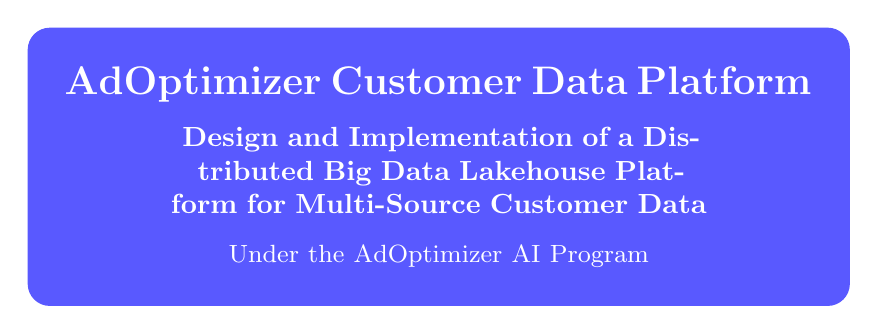
\begin{tikzpicture}
            \node[
                rounded corners=8pt,
                fill=blue!65,
                text=white,
                inner sep=14pt,
                text width=0.78\textwidth,
                align=center
            ] {
                {\Large\bfseries AdOptimizer Customer Data Platform}\\[0.25cm]
                {\normalsize\bfseries Design and Implementation of a Distributed Big Data Lakehouse Platform for Multi-Source Customer Data}\\[0.2cm]
                {\small Under the AdOptimizer AI Program}
            };
        \end{tikzpicture}

        \vfill

        {\bfseries Prepared by}\\
        {\large\bfseries AIT-LAHCEN REDOUAN}

        \vspace{0.8cm}

        {\bfseries Supervised by}\\
        {\bfseries Professor / Academic Supervisor Name}

        \vspace{0.8cm}

        {\bfseries Academic Year: 2025--2026}
    \end{center}
\end{titlepage}

% ============================================================
% Front Matter
% ============================================================
\pagenumbering{roman}
\setcounter{page}{1}

\frontchapter{Dedication}

\vspace*{1.6cm}

\begin{center}
    \begin{minipage}{0.72\textwidth}
        \centering
        {\large\itshape
        To my dear parents,\\[0.45cm]
        for their unconditional love, sacrifices, prayers, and constant support.\\[0.65cm]

        To my family,\\[0.45cm]
        for their encouragement, patience, and confidence throughout this journey.\\[0.65cm]

        To my teachers and mentors,\\[0.45cm]
        for their guidance, inspiration, and valuable advice.\\[0.9cm]

        I dedicate this work with deep gratitude and respect.
        }

        \vspace{1.1cm}

        {\normalsize\itshape AIT-LAHCEN REDOUAN}
    \end{minipage}
\end{center}

\frontchapter{Acknowledgements}
I would like to express my sincere gratitude to my academic supervisor for the guidance, availability, constructive feedback, and encouragement provided throughout this final year project. The advice received helped me clarify the project scope, strengthen the technical choices, and maintain a rigorous engineering approach.

I would also like to thank the academic staff for the knowledge and methodological foundations shared during my Master's program. Their teaching contributed directly to my understanding of data engineering, distributed systems, databases, software development, and reliable information system design.

My appreciation goes to the professional environment that supported the context of this project and helped me understand practical data engineering requirements. Working under the broader AdOptimizer AI initiative allowed me to position this work as a customer data engineering platform, focused on ingestion, distributed storage, lakehouse organization, transformation, quality validation, orchestration, and observability.

I am grateful to my colleagues and classmates for their discussions, shared ideas, and support during this academic journey. I also extend my deepest thanks to my family for their patience, encouragement, and confidence during the long periods of research, implementation, testing, and documentation.

Finally, I would like to thank the members of the jury for the time and attention devoted to evaluating this work. I hope this report clearly reflects the effort invested in designing and implementing a modern, distributed, and production-oriented data engineering platform.

\frontchapter{Abstract}
Modern organizations increasingly rely on data produced from multiple heterogeneous sources, including transactional systems, e-commerce platforms, behavioral event streams, and customer profile datasets. However, transforming these raw inputs into reliable, governed, and analytics-ready data products requires a structured data engineering platform capable of ingestion, storage, distributed processing, validation, orchestration, and monitoring.

This final year project presents the design and implementation of the \textbf{AdOptimizer Customer Data Platform}, a distributed Big Data lakehouse platform developed under the broader AdOptimizer AI program. The platform focuses on building a scalable data engineering foundation for multi-source customer data. It integrates Apache Kafka for ingestion, Hadoop HDFS for distributed storage, Apache Spark for distributed processing, Apache Iceberg and Hive Metastore for lakehouse table management, Trino for SQL exploration, dbt-Spark for transformation modeling, Great Expectations for data quality validation, Apache Airflow for orchestration, and Prometheus with Grafana for observability.

The project demonstrates an end-to-end architecture that transforms raw customer-related datasets into structured lakehouse layers and trusted analytical data products. The implemented solution emphasizes modularity, reproducibility, scalability, data quality, observability, and readiness for future analytics and machine learning use cases.

\textbf{Keywords:} Big Data, Data Engineering, Distributed Systems, Data Lakehouse, Apache Kafka, Hadoop HDFS, Apache Spark, Apache Iceberg, Hive Metastore, Trino, dbt-Spark, Great Expectations, Apache Airflow, Prometheus, Grafana, Data Quality, Observability, Data Governance, Customer Data Platform.

\frontchapter{Résumé}
Les organisations modernes exploitent des donnees issues de sources heterogenes telles que les systemes transactionnels, les plateformes e-commerce, les evenements comportementaux et les donnees de profil client. Cependant, la transformation de ces donnees brutes en produits de donnees fiables, gouvernes et exploitables necessite une plateforme d'ingenierie de donnees structuree, capable d'assurer l'ingestion, le stockage, le traitement distribue, la validation, l'orchestration et la supervision.

Ce projet de fin d'etudes presente la conception et la mise en oeuvre de la plateforme \textbf{AdOptimizer Customer Data Platform}, une plateforme Big Data lakehouse distribuee realisee dans le cadre du programme AdOptimizer AI. Le projet se concentre sur la construction d'une fondation d'ingenierie de donnees scalable pour les donnees client multi-sources. L'architecture integre Apache Kafka pour l'ingestion, Hadoop HDFS pour le stockage distribue, Apache Spark pour le traitement distribue, Apache Iceberg et Hive Metastore pour la gestion des tables lakehouse, Trino pour l'exploration SQL, dbt-Spark pour les transformations, Great Expectations pour la qualite des donnees, Apache Airflow pour l'orchestration, ainsi que Prometheus et Grafana pour l'observabilite.

La solution realisee illustre une chaine de traitement complete permettant de convertir des donnees client brutes en couches lakehouse structurees et en produits de donnees analytiques fiables. Elle met l'accent sur la modularite, la reproductibilite, la scalabilite, la qualite des donnees, l'observabilite et la preparation de futurs cas d'usage analytiques et machine learning.

\textbf{Mots-cles :} Big Data, Ingenierie des donnees, Systemes distribues, Data Lakehouse, Ingestion de donnees, Apache Kafka, Hadoop HDFS, Apache Spark, Apache Iceberg, Hive Metastore, Trino, dbt-Spark, Great Expectations, Apache Airflow, Prometheus, Grafana, Qualite des donnees, Observabilite, Gouvernance des donnees.

% ============================================================
% Planned Table of Contents
% ============================================================
\clearpage
\phantomsection
\chapter*{Table of Contents}
\addcontentsline{toc}{chapter}{Table of Contents}

\begin{center}
    {\Large\bfseries TABLE OF CONTENTS}
\end{center}

\vspace{0.6cm}

\tocfront{DEDICATION}{I}
\tocfront{ACKNOWLEDGEMENTS}{II}
\tocfront{ABSTRACT}{III}
\tocfront{RESUME}{IV}
\tocfront{TABLE OF CONTENTS}{V}
\tocfront{LIST OF FIGURES}{VII}
\tocfront{LIST OF TABLES}{VIII}
\tocfront{LIST OF ACRONYMS AND ABBREVIATIONS}{IX}

\vspace{0.6cm}

\tocunnumbered{GENERAL INTRODUCTION}{1}

\tocchapter{I}{GENERAL PROJECT CONTEXT}{4}
\tocsection{I.1}{Introduction}{5}
\tocsection{I.2}{Host Organization and Project Environment}{5}
\tocsubsection{I.2.1}{Company Context and Digital Transformation Needs}{6}
\tocsubsection{I.2.2}{Data-Driven Decision-Making Challenges}{7}
\tocsubsection{I.2.3}{AdOptimizer AI as the Global Program}{8}
\tocsection{I.3}{Target Project Presentation}{9}
\tocsubsection{I.3.1}{AdOptimizer Customer Data Platform Principle}{9}
\tocsubsection{I.3.2}{Problem Statement}{10}
\tocsubsection{I.3.3}{Project Objectives}{12}
\tocsubsection{I.3.4}{Project Scope and Boundaries}{13}
\tocsubsection{I.3.5}{Expected Outcomes}{15}
\tocsubsection{I.3.6}{Project Planning and Methodology}{16}
\tocsection{I.4}{Conclusion}{17}

\tocchapter{II}{STATE OF THE ART AND THEORETICAL BACKGROUND}{18}
\tocsection{II.1}{Introduction}{19}
\tocsection{II.2}{Big Data Fundamentals}{19}
\tocsubsection{II.2.1}{Emergence and Evolution of Big Data}{20}
\tocsubsection{II.2.2}{The Five Vs of Big Data}{21}
\tocsubsection{II.2.3}{Distributed Storage and Distributed Processing}{23}
\tocsection{II.3}{Big Data Architectures}{25}
\tocsubsection{II.3.1}{Traditional Data Warehouse Architecture}{25}
\tocsubsection{II.3.2}{Data Lake Architecture}{27}
\tocsubsection{II.3.3}{Data Lakehouse Architecture}{29}
\tocsubsection{II.3.4}{Lambda Architecture}{31}
\tocsubsection{II.3.5}{Kappa Architecture}{33}
\tocsubsection{II.3.6}{Comparison Between Lambda and Kappa}{35}
\tocsection{II.4}{Technology Watch}{37}
\tocsubsection{II.4.1}{Apache Kafka for Data Ingestion}{37}
\tocsubsection{II.4.2}{Hadoop HDFS for Distributed Storage}{38}
\tocsubsection{II.4.3}{Apache Spark for Distributed Processing}{39}
\tocsubsection{II.4.4}{Apache Iceberg and Hive Metastore for Lakehouse Tables}{40}
\tocsubsection{II.4.5}{Trino, dbt-Spark, Great Expectations, and Airflow}{41}
\tocsection{II.5}{Conclusion}{41}

\tocchapter{III}{REQUIREMENTS ANALYSIS AND SYSTEM DESIGN}{42}
\tocsection{III.1}{Introduction}{43}
\tocsection{III.2}{Requirements Analysis}{43}
\tocsubsection{III.2.1}{Functional Requirements}{44}
\tocsubsection{III.2.2}{Non-Functional Requirements}{46}
\tocsubsection{III.2.3}{Data Quality and Governance Requirements}{48}
\tocsubsection{III.2.4}{Observability and Operational Requirements}{49}
\tocsection{III.3}{Conceptual Design}{50}
\tocsubsection{III.3.1}{Actors and Use Cases}{50}
\tocsubsection{III.3.2}{Data Source Analysis}{52}
\tocsubsection{III.3.3}{Lakehouse Layering Strategy}{54}
\tocsection{III.4}{Global Architecture}{56}
\tocsubsection{III.4.1}{End-to-End Data Flow}{57}
\tocsubsection{III.4.2}{Tool Interaction and Integration}{59}
\tocsubsection{III.4.3}{Deployment and Distribution View}{61}
\tocsection{III.5}{Conclusion}{62}

\tocchapter{IV}{IMPLEMENTATION OF THE DISTRIBUTED LAKEHOUSE PLATFORM}{63}
\tocsection{IV.1}{Introduction}{64}
\tocsection{IV.2}{Development Environment Preparation}{64}
\tocsubsection{IV.2.1}{Project Repository Organization}{65}
\tocsubsection{IV.2.2}{Environment Variables and Configuration Strategy}{66}
\tocsubsection{IV.2.3}{Docker-Based Service Deployment}{67}
\tocsection{IV.3}{Streaming and Ingestion Layer}{68}
\tocsubsection{IV.3.1}{Kafka Broker and Kafka UI Setup}{68}
\tocsubsection{IV.3.2}{Dataset-Specific Producers}{69}
\tocsubsection{IV.3.3}{Topic Reset and Idempotent Reprocessing}{71}
\tocsection{IV.4}{Distributed Storage Layer}{72}
\tocsubsection{IV.4.1}{HDFS Namenode and Datanode Setup}{72}
\tocsubsection{IV.4.2}{Bronze Zone Directory Structure}{73}
\tocsubsection{IV.4.3}{Landing Raw Files from Kafka into HDFS}{74}
\tocsection{IV.5}{Distributed Processing and Lakehouse Table Layer}{76}
\tocsubsection{IV.5.1}{Spark Cluster Setup}{76}
\tocsubsection{IV.5.2}{Hive Metastore and Iceberg Catalog}{78}
\tocsubsection{IV.5.3}{Spark Raw Table Loading}{80}
\tocsubsection{IV.5.4}{Trino SQL Query Service}{82}
\tocsection{IV.6}{Transformation Layer with dbt-Spark}{83}
\tocsubsection{IV.6.1}{Staging Models}{84}
\tocsubsection{IV.6.2}{Intermediate Models}{86}
\tocsubsection{IV.6.3}{Analytics Models}{88}
\tocsection{IV.7}{Data Quality Layer with Great Expectations}{89}
\tocsection{IV.8}{Orchestration with Apache Airflow}{90}
\tocsection{IV.9}{Monitoring with Prometheus and Grafana}{91}
\tocsection{IV.10}{Conclusion}{92}

\tocchapter{V}{CASE STUDY: MULTI-SOURCE CUSTOMER DATA LAKEHOUSE}{93}
\tocsection{V.1}{Introduction}{94}
\tocsection{V.2}{Source Dataset Description}{94}
\tocsubsection{V.2.1}{Customer Personality Dataset}{95}
\tocsubsection{V.2.2}{E-commerce Customer Churn Dataset}{96}
\tocsubsection{V.2.3}{RetailRocket Events Dataset}{97}
\tocsubsection{V.2.4}{Online Retail Dataset}{98}
\tocsection{V.3}{Data Ingestion Execution}{99}
\tocsection{V.4}{Bronze Layer Validation}{100}
\tocsection{V.5}{Raw Iceberg Table Construction}{101}
\tocsection{V.6}{Analytical Data Products}{102}
\tocsection{V.7}{Future AI and Machine Learning Readiness}{103}
\tocsection{V.8}{Conclusion}{104}

\tocchapter{VI}{TESTING, VALIDATION, AND PERFORMANCE EVALUATION}{105}
\tocsection{VI.1}{Introduction}{106}
\tocsection{VI.2}{Service Readiness Tests}{106}
\tocsubsection{VI.2.1}{HDFS Readiness}{107}
\tocsubsection{VI.2.2}{Hive Metastore Readiness}{107}
\tocsubsection{VI.2.3}{Spark and Spark Thrift Readiness}{108}
\tocsubsection{VI.2.4}{Trino Query Service Readiness}{109}
\tocsection{VI.3}{Data Quality Validation}{110}
\tocsubsection{VI.3.1}{Raw Lakehouse Quality Checks}{110}
\tocsubsection{VI.3.2}{Transformation Quality Checks}{111}
\tocsection{VI.4}{End-to-End Pipeline Validation}{112}
\tocsection{VI.5}{Monitoring Dashboard Validation}{114}
\tocsection{VI.6}{Performance Evaluation Approach}{116}
\tocsubsection{VI.6.1}{Local Execution Baseline}{116}
\tocsubsection{VI.6.2}{Distributed Deployment Benchmark Plan}{117}
\tocsection{VI.7}{Conclusion}{118}

\tocchapter{VII}{DEPLOYMENT STRATEGY AND SCALABILITY PERSPECTIVE}{119}
\tocsection{VII.1}{Introduction}{120}
\tocsection{VII.2}{Target Multi-Machine Deployment Context}{120}
\tocsection{VII.3}{Service Distribution Strategy}{121}
\tocsubsection{VII.3.1}{Coordination, Ingestion, and Orchestration Node}{122}
\tocsubsection{VII.3.2}{Storage and Catalog Node}{123}
\tocsubsection{VII.3.3}{Processing and Query Node}{123}
\tocsection{VII.4}{Scalability and Fault-Tolerance Considerations}{124}
\tocsection{VII.5}{Security and DataSecOps Considerations}{124}
\tocsection{VII.6}{Conclusion}{124}

\tocunnumbered{GENERAL CONCLUSION AND PERSPECTIVES}{125}

\tocunnumbered{REFERENCES}{127}

\tocchapter{A}{APPENDICES}{128}
\tocsection{A.1}{Technical Runbook}{128}
\tocsection{A.2}{Environment Variables}{129}
\tocsection{A.3}{Docker Services and Ports}{129}
\tocsection{A.4}{Airflow DAG Execution Order}{130}
\tocsection{A.5}{Monitoring Dashboard Inventory}{130}

\end{document}
